\documentclass{article}[11pt,subeqn]

\title{Twin Descriptives...}
\author{Sonia Bhalotra\thanks{The University of Essex.  Contact: srbhal@essex.ac.uk} 
\and Damian Clarke\thanks{The University of Oxford.  Contact: damian.clarke@economics.ox.ac.uk}}
\date{\today}

\usepackage[capposition=top]{floatrow}
\usepackage{url}
\usepackage{longtable}
\usepackage{booktabs}
\usepackage{rotating}
\usepackage{dcolumn}
\usepackage{color}
\pagecolor{white}
\usepackage{pdfpages}
\usepackage{lastpage}
\usepackage{lscape}
\usepackage{setspace}
\usepackage{amsmath}
\usepackage{amssymb}
\usepackage{breqn}
\usepackage{appendix}
\usepackage{natbib}
\bibliographystyle{abbrvnat}
\bibpunct{(}{)}{;}{a}{,}{,}

\usepackage{epsfig}
\usepackage{epstopdf}
\usepackage{multirow}


\usepackage{wrapfig}
\usepackage{blindtext}

\setlength\topmargin{-0.375in}
\setlength\textheight{8.8in}
\setlength\textwidth{5.8in}
\setlength\oddsidemargin{0.4in}
\setlength\evensidemargin{-0.5in}
\setlength\parindent{0.25in}
\setlength\parskip{0.25in}


\bibliographystyle{abbrvnat}
\bibpunct{(}{)}{;}{a}{,}{,}

\newcommand\independent{\protect\mathpalette{\protect\independenT}{\perp}}
\def\independenT#1#2{\mathrel{\rlap{$#1#2$}\mkern2mu{#1#2}}}

\usepackage{changepage}% http://ctan.org/pkg/changepage
\makeatletter
\newenvironment{chapabstract}{%
    \begin{center}%
      \bfseries Abstract
    \end{center}}%
   {\par}
\makeatother


\newcommand{\twinfolder}{./../../Twins/Scientific}

\begin{document}
\begin{spacing}{1.4}

\maketitle



\newpage
\section*{Figures}
\begin{figure}[htpb!]
\centering
\begin{subfigure}{.5\textwidth}
  \centering
  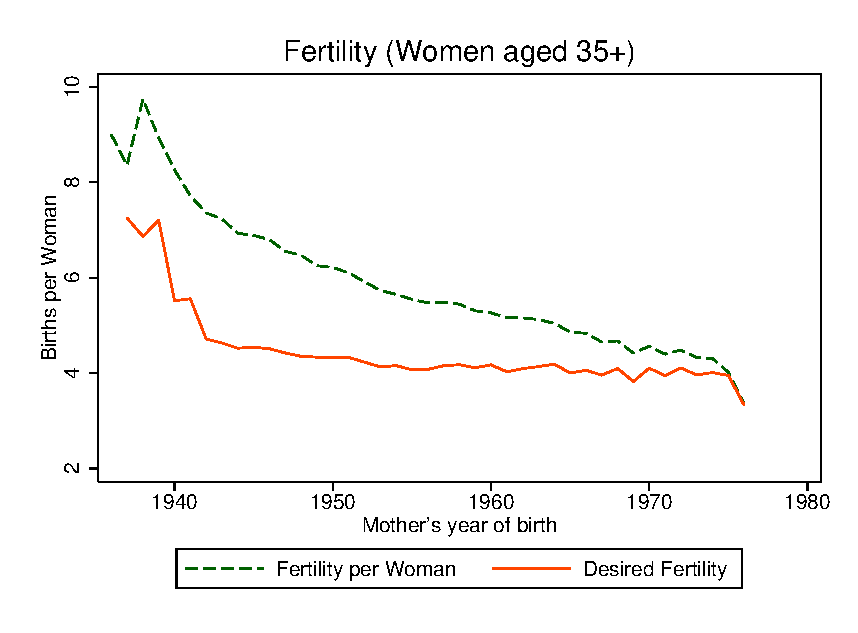
\includegraphics[scale=0.53]{\twinfolder/Figures/ferttrend_35_all.eps}
  \caption{Trends in Fertility}
  \label{TWINfig:fertrend}
\end{subfigure}%
\begin{subfigure}{.5\textwidth}
  \centering
  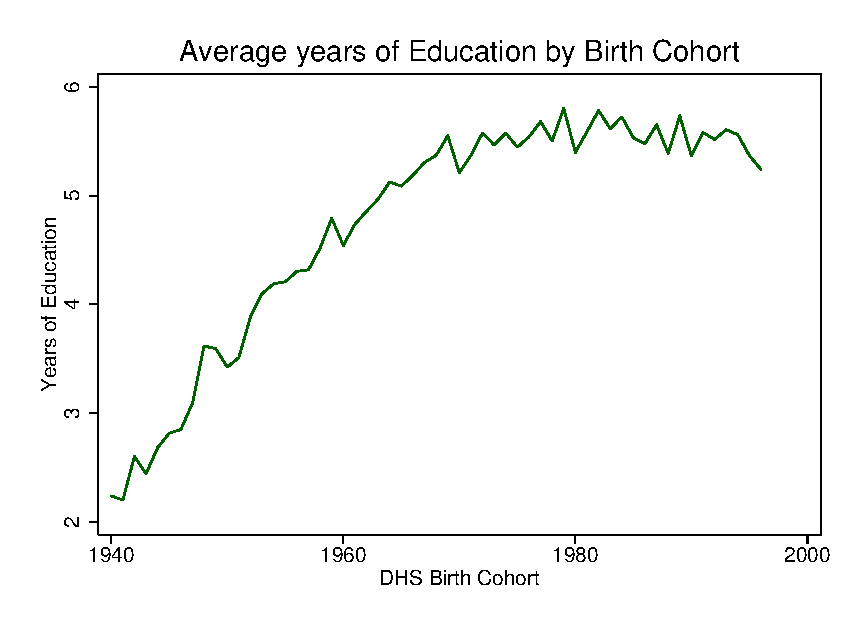
\includegraphics[scale=0.52]{\twinfolder/Figures/eductrend_all.eps}
  \caption{Trend in Education}
  \label{TWINfig:eductrend}
\end{subfigure}
\caption{Education and Fertility}
\label{TWINfig:trends}
\floatfoot{Note to figure \ref{TWINfig:trends}: Cohorts are made up of all individuals 
from the DHS who are over 35 years (for fertility), and over 15 years (for education).  
In each case the sample is restricted to those who have approximately completed fertility 
and education respectively.}
\end{figure}
\vspace{1cm}

\begin{figure}[htpb!]
\begin{center}
\caption{Proportion of Twins by Birth Order}
\label{TWINfig:bord}
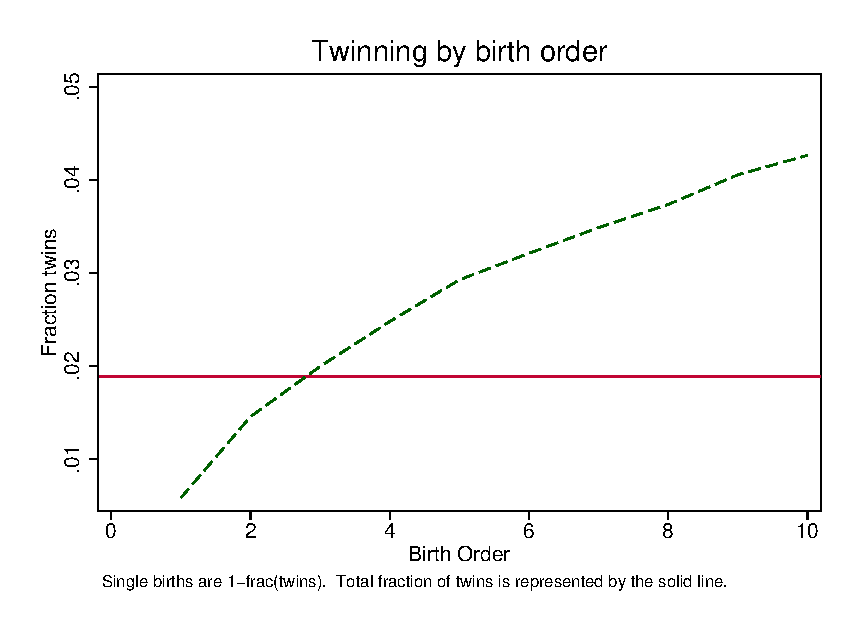
\includegraphics[scale=0.92]{\twinfolder/Figures/twinbybord.eps} 
\end{center}
\end{figure}

\begin{figure}[htpb!]
\begin{center}
\caption{Twin Births and Total Fertility}
\label{TWINfig:births}
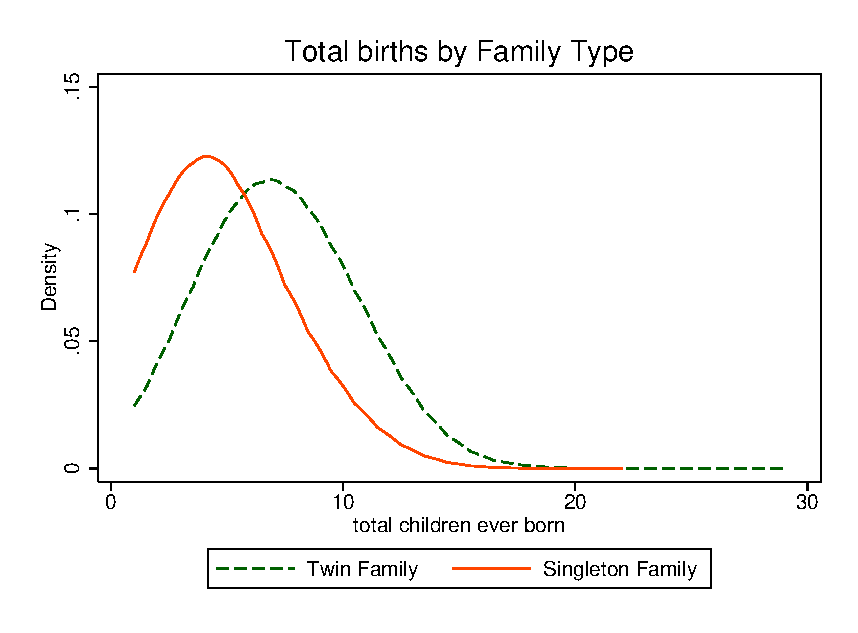
\includegraphics[scale=0.92]{\twinfolder/Figures/famsize.eps} 
\end{center}
\end{figure}

\begin{figure}[htpb!]
\begin{center}
\caption{Distribution of Ideal Family Size}
\label{TWINfig:ideal}
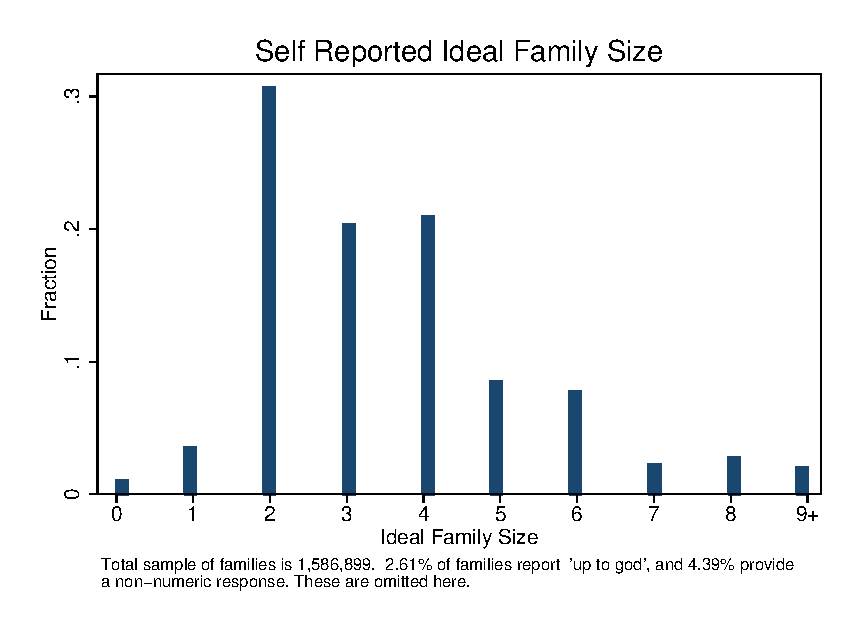
\includegraphics[scale=0.92]{\twinfolder/Figures/idealfamsize.eps} 
\end{center}
\end{figure}

\begin{figure}[htpb!]
\begin{center}
\caption{Ideal and Actual Fertility}
\label{TWINfig:idealactual}
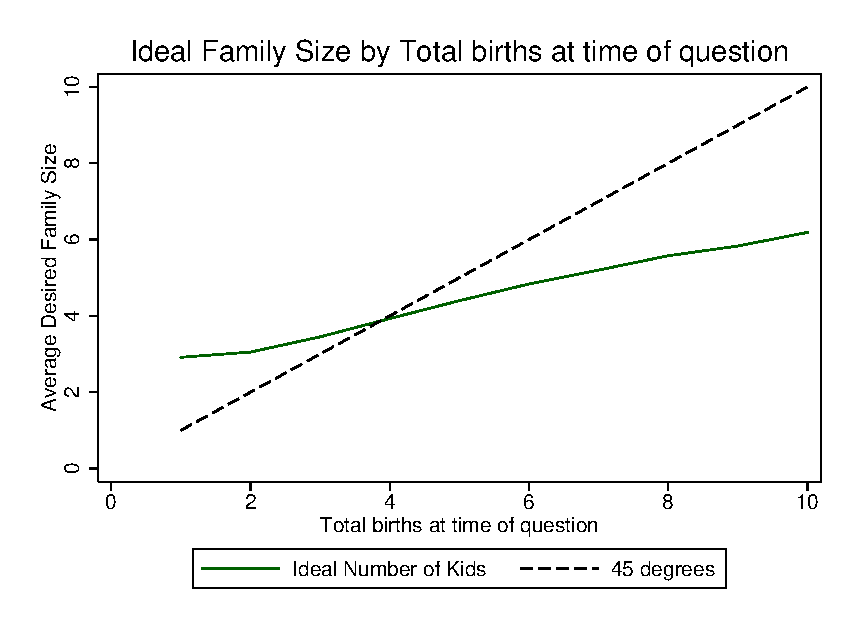
\includegraphics[scale=0.92]{\twinfolder/Figures/idealfam_fert.eps} 
\end{center}
\end{figure}

\begin{figure}[htpb!]
\begin{center}
\caption{Relaxing Strict Exogeneity (two plus)}
\label{TWINfig:ltz2}
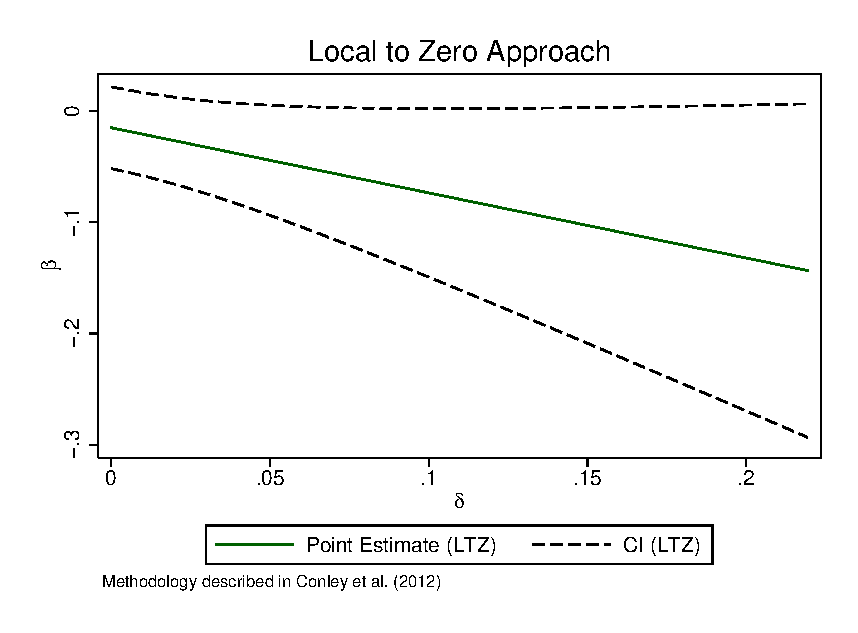
\includegraphics[scale=0.88]{\twinfolder/Figures/LTZ_two.eps}
\vspace{-8mm}
\floatfoot{Note to figure \ref{TWINfig:ltz2}: See note to Figure \ref{TWINfig:ltz3}}
\end{center}
\end{figure}

\begin{figure}[htpb!]
\begin{center}
\caption{Relaxing Strict Exogeneity (three plus)}
\label{TWINfig:ltz3}
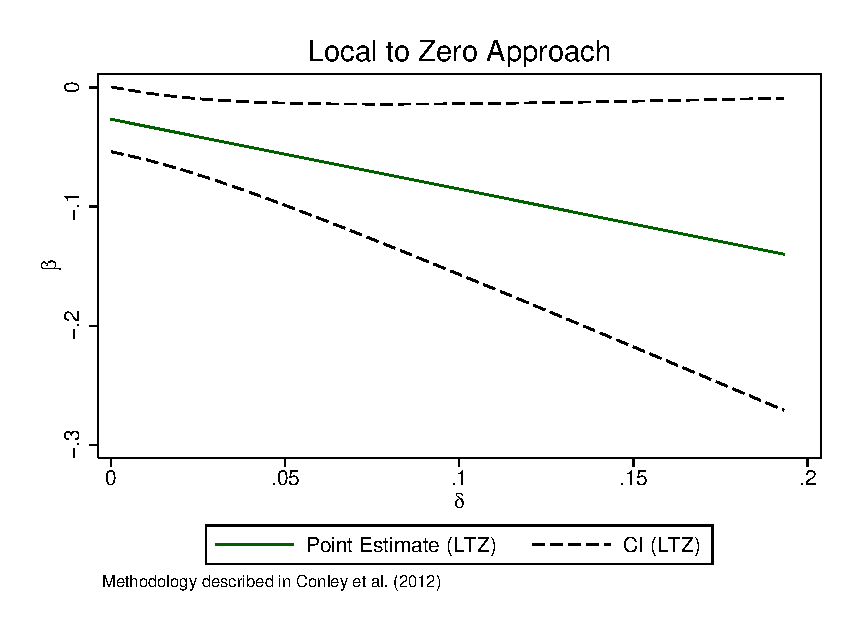
\includegraphics[scale=0.88]{\twinfolder/Figures/LTZ_three.eps} 
\floatfoot{Note to figure \ref{TWINfig:ltz3}: Confidence intervals and point estimates 
are calculated according to \citet{Conleyetal2012}.  Estimates reflect a range of priors 
regarding the validity of the exclusion restriction required to consistently estimate 
$\hat\beta_{fert}$ using twinning in a 2SLS framework.  The local to zero (LTZ) 
approach applied here assumes that $\gamma$, the sign on the instrument when included
in the first stage, is distributed $\gamma\sim U(0,\delta)$.  Further discussion 
is provided in the body of the text and table \ref{TWINtab:Conley}.}
\end{center}
\end{figure}

\clearpage

\section*{Tables}
\begin{table}[htpb!]\caption{Summary Statistics} 
\label{TWINtab:sumstats}\begin{center}\scalebox{0.99}{\begin{tabular}{lccccc}
\toprule \toprule 
&\multicolumn{2}{c}{Low Income}&\multicolumn{2}{c}{Middle Income}\\ 
\cmidrule(r){2-3} \cmidrule(r){4-5}
& Single & Twins & Single & Twins & All \\ \midrule 
\textsc{Fertility} & & & & & \\ 
Fertility&3.749&6.223&3.412&5.584&3.689\\
&(2.392)&(2.622)&(2.308)&(2.687)&(2.406)\\
Desired Family Size&4.193&5.328&3.380&4.190&3.921\\
&(2.530)&(2.885)&(2.130)&(2.555)&(2.440)\\
Fraction Twin & \multicolumn{2}{c}{  0.0200}& \multicolumn{2}{c}{  0.0179 } &  0.0191\\
& \multicolumn{2}{c}{(0.1402)}& \multicolumn{2}{c}{(0.1326)} & (0.1370)\\
Birth Order Twin & \multicolumn{2}{c}{   4.664}& \multicolumn{2}{c}{   4.016 }&   4.410\\
& \multicolumn{2}{c}{(2.465)}& \multicolumn{2}{c}{(2.374)}& (2.450)\\
\textsc{Mother's Characteristics}&&&&&\\ Age
&31.22&34.52&32.32&35.61&31.72\\
&(8.238)&(7.381)&(8.356)&(7.428)&(8.293)\\
Education&3.859&3.222&6.690&5.906&4.885\\
&(4.327)&(3.991)&(4.795)&(5.023)&(4.706)\\
Height&155.5&157.6&155.6&157.2&155.6\\
&(7.093)&(7.065)&(6.966)&(6.945)&(7.053)\\
BMI&21.90&22.50&25.90&26.63&23.39\\
&(4.027)&(4.175)&(5.118)&(5.512)&(4.867)\\
Pr(BMI)$<$18.5&0.175&0.125&0.0346&0.0276&0.122\\
&(0.380)&(0.331)&(0.183)&(0.164)&(0.327)\\
Actual Births$>$Desired&0.310&0.526&0.324&0.575&0.321\\
&(0.463)&(0.499)&(0.468)&(0.494)&(0.467)\\
\textsc{Children's Outcomes}&&&&&\\ Education (Years)
&3.660&3.204&5.445&5.043&4.446\\
&(3.576)&(3.293)&(3.867)&(3.760)&(3.810)\\
Education (Z-Score)&-0.00843&-0.0156&0.0119&-0.0428&0.000144\\
&(1.001)&(0.963)&(0.998)&(0.987)&(1.000)\\
No Education (Percent)&0.207&0.222&0.0649&0.0786&0.144\\
&(0.405)&(0.416)&(0.246)&(0.269)&(0.351)\\
Infant Mortality&0.0158&0.0917&0.00946&0.0497&0.0141\\
&(0.125)&(0.289)&(0.0968)&(0.217)&(0.118)\\
Child Mortality&0.0239&0.108&0.0122&0.0535&0.0199\\
&(0.153)&(0.310)&(0.110)&(0.225)&(0.140)\\
\midrule
Number of Countries & 39&39  & 28&28  & 67 \\
Number of Children &2,231,844 &45,654 &1,614,358 &29,430 & 3,921,286 \\
Number of Mothers &875,587 &12,908 &653,969 &8,605 & 1,586,899 \\
\midrule
\multicolumn{6}{p{13.2cm}}{\begin{footnotesize}\textsc{Notes:}  Group means are presented with standard deviation below in parenthesis.  Education is reported as total years attained, and Z-score presents educational attainment relative to country and cohort (mean 0, std deviation 1).  Infant mortality refers to the proportion of children who die before 1 year of age,  while child mortality refers to the proportion who die before 5 years.  Maternal height is reported in cm, and BMI is weight in kg over height in metres squared.  Summary statistics are for the full sample of 1,586,899
 mothers responding to any publicly available DHS survey.  For a full list of country and years of survey, see appendix table \ref{TWINtab:countries}.\end{footnotesize}} \\ \bottomrule \end{tabular}}\end{center}\end{table}

\begin{table}[htbp]\centering
\def\sym#1{\ifmmode^{#1}\else\(^{#1}\)\fi}
\caption{Test of Balance of Observables: Twins versus Non-twins \label{TWINtab:comp}}
\vspace{5mm}\begin{tabular}{l*{1}{ccc}}
\toprule\toprule & Non-Twin & Twin & Diff.\\
                    &        Family&        Family&      (Diff. SE)         \\
\midrule
Total Fertilty      &       4.460&       6.787&      -2.327\sym{***}\\
                    &            &            &    (0.0255)         \\
Desired Fertility   &       4.451&       5.566&      -1.116\sym{***}\\
                    &            &            &    (0.0312)         \\
Age First Birth     &       19.15&       18.98&       0.170\sym{***}\\
                    &            &            &    (0.0424)         \\
Mother's Education  &       4.269&       3.351&       0.918\sym{***}\\
                    &            &            &    (0.0523)         \\
Father's Education  &       5.510&       4.710&       0.800\sym{***}\\
                    &            &            &    (0.0584)         \\
Mother's Height     &       156.1&       157.8&      -1.716\sym{***}\\
                    &            &            &    (0.0839)         \\
Pr(BMI $<$ 18.5)    &       0.120&      0.0937&      0.0265\sym{***}\\
                    &            &            &   (0.00382)         \\
Number of Antenatal Checks&       3.901&       3.815&      0.0860\sym{*}  \\
                    &            &            &    (0.0374)         \\
Prenatal care (doctor)&       0.313&       0.211&       0.102\sym{***}\\
                    &            &            &   (0.00544)         \\
Prenatal care (nurse)&       0.452&       0.521&     -0.0690\sym{***}\\
                    &            &            &   (0.00588)         \\
Prenatal care (none)&       0.193&       0.183&     0.00979\sym{*}  \\
                    &            &            &   (0.00466)         \\
Mother's Age        &       25.53&       27.61&      -2.077\sym{***}\\
                    &            &            &    (0.0565)         \\
Child Mortality     &      0.0102&      0.0255&     -0.0153\sym{***}\\
                    &            &            &  (0.000912)         \\
Infant Mortality    &     0.00580&      0.0170&     -0.0112\sym{***}\\
                    &            &            &  (0.000606)         \\
Wealth Quintile 1   &       0.259&       0.274&     -0.0154\sym{**} \\
                    &            &            &   (0.00518)         \\
Wealth Quintile 2   &       0.220&       0.227&    -0.00691         \\
                    &            &            &   (0.00490)         \\
Wealth Quintile 3   &       0.198&       0.201&    -0.00351         \\
                    &            &            &   (0.00471)         \\
Wealth Quintile 4   &       0.176&       0.175&    0.000653         \\
                    &            &            &   (0.00450)         \\
Wealth Quintile 5   &       0.148&       0.123&      0.0252\sym{***}\\
                    &            &            &   (0.00418)         \\
\midrule\midrule


\multicolumn{4}{p{10.4cm}}{\begin{footnotesize}\textsc{Notes:} Education measured in years, mother's height in centimetres, and BMI is weight in kilograms over height in metres squared.  Diff. SE is calculated using a two-tailed t-test. $^{*}$p$<$0.1; $^{**}$p$<$0.05; $^{***}$p$<$0.01\end{footnotesize}}
\\\bottomrule\normalsize\end{tabular}\end{table} 


\begin{table}[htpb!]
\caption{Test of hypothesis that women who bear twins have better prior health}\label{TWINtab:IMR}\begin{center}\begin{tabular}{lccc}
\toprule \toprule 
\textsc{Infant Mortality (per 100 births)}& Base & +S\&H & Observations \\ \midrule 
\begin{footnotesize}\end{footnotesize}& 
\begin{footnotesize}\end{footnotesize}& 
\begin{footnotesize}\end{footnotesize}& 
\begin{footnotesize}\end{footnotesize}\\ 
Treated (2+)\hspace{5mm}\hspace{5mm}\hspace{5mm}\hspace{5mm}\hspace{5mm}\hspace{5mm}&-2.065***&-2.110***&503785\\
&(0.212)&(0.213)&\\
Treated (3+)\hspace{5mm}&-4.619***&-4.632***&686931\\
&(0.201)&(0.201)&\\
Treated (4+)&-4.257***&-4.243***&676303\\
&(0.183)&(0.183)&\\
Treated (5+)&-3.353***&-3.324***&587919\\
&(0.183)&(0.183)&\\
\midrule\multicolumn{4}{p{12.1cm}}{\begin{footnotesize}\textsc{Notes:} The sample for these regressions consist of all children who have been entirely exposed to the risk of infant mortality (ie those over 1 year of age). Subsamples 2+, 3+, 4+ and 5+ are generated to allow comparison of children born at similar birth orders.  For a full description of these groups see the the body of the paper or notes to table \ref{TWINtab:IVAll}. Treated=1 refers to children who are born before a twin while Treated=0 refers to children of similar birth orders not born before a twin.  Base and S+H controls are described in table \ref{TWINtab:IVAll}.$^{*}$p$<$0.1; $^{**}$p$<$0.05; $^{***}$p$<$0.01 
\end{footnotesize}} \\ \bottomrule 
\end{tabular}\end{center}\end{table}

\begin{landscape}\begin{table}[!htbp] \centering 
\caption{OLS Estimates of the Q-Q Trade-off} 
 \vspace{4mm}\label{TWINtab:OLS} 
\begin{tabular}{lcccccc} \toprule \toprule 
&Base&+&+&Desired&Altonji&Altonji\\
&Controls&Socioec&Health&&Ratio 1&Ratio 2\\\midrule
\textsc{Panel A: All Countries}&&&&&&\\
Fertility &-0.115***&-0.0777***&-0.0751***&-0.0717***&2.083&1.882\\
&(0.000815)&(0.000776)&(0.000771)&(0.000838)&&\\
Fertility$\times$desire&&&&-0.00558***&&\\
&&&&(0.000495)&&\\
&&&&&&\\
Observations &1,334,874&1,334,874&1,334,874&1,334,874&&\\
R$^2$&0.094&0.161&0.167&0.168&&\\\midrule
\textsc{Panel B: Low Income}&&&&&&\\
Fertility &-0.110***&-0.0734***&-0.0712***&-0.0668***&2.005&1.835\\
&(0.00106)&(0.000988)&(0.000975)&(0.00107)&&\\
Fertility$\times$desire&&&&-0.00674***&&\\
&&&&(0.000608)&&\\
&&&&&&\\
Observations &831,476&831,476&831,476&831,476&&\\
R$^2$&0.091&0.171&0.181&0.182&&\\\midrule
\textsc{Panel C: Middle Income}&&&&&&\\
Fertility &-0.125***&-0.0875***&-0.0854***&-0.0839***&2.333&2.157\\
&(0.00128)&(0.00126)&(0.00126)&(0.00134)&&\\
Fertility$\times$desire&&&&-0.00266***&&\\
&&&&(0.000846)&&\\
&&&&&&\\
Observations &503,398&503,398&503,398&503,398&&\\
R$^2$&0.106&0.154&0.156&0.156&&\\\hline\hline
\multicolumn{7}{p{15.8cm}}{\begin{footnotesize}\textsc{Notes:} Base controls consist of child gender, mother's age and age squared mother's age at first birth, child age, country, and year of birth dummies.  Socioeconomic augments `Base' to include mother's education and education squared, and Health includes mother's height and BMI. ``Desire'' takes 1 if the child is born before the family reaches it's desired size, and 0 if the child is born after the desired size is reached. The \citet{Altonjietal2005} ratio determines how important unobservable factors must be compared with included observables to imply that the true effect of fertilty on educational attainment is equal to zero.  Ratio 1 compares no controls to socioeconomic controls, while ratio 2 compares no controls to socioeconomic and health controls. Standard errors are clustered at the level of the mother.
$^{*}$p$<$0.1; $^{**}$p$<$0.05; $^{***}$p$<$0.01\end{footnotesize}}\\  
\bottomrule \normalsize\end{tabular}\end{table}\end{landscape} 


\begin{table}[!htbp] \centering 
\caption{Instrumental Variables Estimates: Two Plus} 
\label{TWINtab:IVTwoplus} 
\begin{tabular}{lcccc} \toprule \toprule 
&Base&&&\\
&Controls&Socioec&Health&Obs.\\\midrule
\multicolumn{5}{l}{\textsc{Pre-Twins}}\\ 
&&&&\\
\multicolumn{5}{l}{\textbf{All Families}}\\ 
Fertility&0.006&-0.026&-0.026&249,536\\
         &(0.029)&(0.027)&(0.026)&\\
&&&&\\
\multicolumn{5}{l}{\textbf{Low-Income Countries}}\\ 
Fertility&0.035&0.008&0.012&149,602\\
         &(0.034)&(0.032)&(0.031)&\\
&&&&\\
\multicolumn{5}{l}{\textbf{Middle-Income Countries}}\\ 
Fertility&-0.065&-0.087*&-0.093**&99,934\\
         &(0.053)&(0.049)&(0.047)&\\
&&&&\\
\multicolumn{5}{l}{\textbf{Desired-Threshold}}\\ 
Fertility&0.007&-0.025&-0.027&249,536\\
         &(0.035)&(0.031)&(0.030)&\\
Fertility$\times$desire&-0.001&0.001&0.000&\\
         &(0.014)&(0.013)&(0.013)&\\
\midrule\multicolumn{5}{l}{\textsc{Twins and Pre-Twins}}\\ 
&&&&\\
\multicolumn{5}{l}{\textbf{All Families}}\\ 
Fertility&-0.021&-0.073***&-0.078***&488,815\\
         &(0.024)&(0.021)&(0.020)&\\
\midrule\multicolumn{5}{l}{\textsc{First Stage (Pre-Twins)}}\\ 
&&&&\\
\multicolumn{5}{l}{\textbf{All Families}}\\ 
Twins&0.776***&0.821***&0.822***&249,536\\
         &(0.031)&(0.029)&(0.028)&\\
\hline\multicolumn{5}{p{10.0cm}}{\begin{footnotesize}\textsc{Notes:} Two-plus refers to all first-born children in families with two or more children.  Each cell presents the coefficient of a 2SLS regression where fertility is instrumented by twinning at birth order two.  Base controls include child age, mother's age, and mother's age at birth fixed effects plus country and year-of-birth FEs.  The sample is made up of all children aged between 6-18 years from families in the DHS who fulfill two-plus requirements. First-stage results in the final panel correspond to the second stage in row 1.  Full first stage results for each row are available in table \ref{TWINtab:FS}. Standard errors are clustered by mother. 
$^{*}$p$<$0.1; $^{**}$p$<$0.05; $^{***}$p$<$0.01\end{footnotesize}}
\\\bottomrule\normalsize\end{tabular}\end{table} 


\begin{table}[!htbp] \centering 
\caption{Instrumental Variables Estimates: Three Plus} 
\label{TWINtab:IVThreeplus} 
\begin{tabular}{lcccc} \toprule \toprule 
&Base&&&\\
&Controls&Socioec&Health&Obs.\\\midrule
\multicolumn{5}{l}{\textsc{Pre-Twins}}\\ 
&&&&\\
\multicolumn{5}{l}{\textbf{All Families}}\\ 
Fertility&-0.010&-0.038*&-0.042**&390,985\\
         &(0.023)&(0.021)&(0.021)&\\
&&&&\\
\multicolumn{5}{l}{\textbf{All Families (bord dummies)}}\\ 
Fertility&-0.010&-0.038*&-0.042**&390,985\\
         &(0.023)&(0.021)&(0.020)&\\
&&&&\\
\multicolumn{5}{l}{\textbf{Low-Income Countries}}\\ 
Fertility&0.006&-0.029&-0.034&244,928\\
         &(0.029)&(0.026)&(0.025)&\\
&&&&\\
\multicolumn{5}{l}{\textbf{Middle-Income Countries}}\\ 
Fertility&-0.045&-0.061*&-0.064*&146,057\\
         &(0.039)&(0.035)&(0.035)&\\
&&&&\\
\multicolumn{5}{l}{\textbf{Desired-Threshold}}\\ 
Fertility&0.001&-0.044*&-0.047**&390,985\\
         &(0.027)&(0.024)&(0.024)&\\
Fertility$\times$desire&-0.011&0.002&0.001&\\
         &(0.010)&(0.009)&(0.009)&\\
\midrule\multicolumn{5}{l}{\textsc{Twins and Pre-Twins}}\\ 
&&&&\\
\multicolumn{5}{l}{\textbf{All Families}}\\ 
Fertility&-0.025&-0.066***&-0.071***&584,566\\
         &(0.020)&(0.018)&(0.018)&\\
&&&&\\
\multicolumn{5}{l}{\textbf{All Families (bord dummies)}}\\ 
Fertility&-0.020&-0.054***&-0.058***&584,566\\
         &(0.021)&(0.019)&(0.018)&\\
\midrule\multicolumn{5}{l}{\textsc{First Stage (Pre-Twins)}}\\ 
&&&&\\
\multicolumn{5}{l}{\textbf{All Families}}\\ 
Twins&0.796***&0.821***&0.824***&390,985\\
         &(0.027)&(0.026)&(0.026)&\\
\hline\multicolumn{5}{p{10cm}}{\begin{footnotesize}\textsc{Notes:} Three-plus refers to all first- and second-born children in families with three or more children.  Each cell presents the coefficient of a 2SLS regression where fertility is instrumented by twinning at birth order three.  Base controls include child age, mother's age, and mother's age at birth fixed effects plus country and year-of-birth FEs.  The sample is made up of all children aged between 6-18 years from families in the DHS who fulfill three-plus requirements. Birth order dummies are included only if explicitly stated.  First-stage results in the final panel correspond to the second stage in row 1.  Full first stage results for each row are available in table \ref{TWINtab:FS}. Standard errors are clustered by mother. 
$^{*}$p$<$0.1; $^{**}$p$<$0.05; $^{***}$p$<$0.01\end{footnotesize}}
\\\bottomrule\normalsize\end{tabular}\end{table} 


\begin{table}[!htbp] \centering 
\caption{Instrumental Variables Estimates: Four Plus} 
\label{TWINtab:IVFourplus} 
\begin{tabular}{lcccc} \toprule \toprule 
&Base&&&\\
&Controls&Socioec&Health&Obs.\\\midrule
\multicolumn{5}{l}{\textsc{Pre-Twins}}\\ 
&&&&\\
\multicolumn{5}{l}{\textbf{All Families}}\\ 
Fertility&-0.017&-0.036&-0.035*&385,389\\
         &(0.025)&(0.023)&(0.021)&\\
&&&&\\
\multicolumn{5}{l}{\textbf{Low-Income Countries}}\\ 
Fertility&-0.011&-0.031&-0.024&246,622\\
         &(0.029)&(0.027)&(0.025)&\\
&&&&\\
\multicolumn{5}{l}{\textbf{Middle-Income Countries}}\\ 
Fertility&-0.027&-0.048&-0.054&138,767\\
         &(0.043)&(0.040)&(0.037)&\\
&&&&\\
\multicolumn{5}{l}{\textbf{Desired-Threshold}}\\ 
Fertility&-0.003&-0.017&-0.020&385,389\\
         &(0.027)&(0.023)&(0.023)&\\
Fertility$\times$desire&-0.012&-0.012&-0.013*&\\
         &(0.008)&(0.007)&(0.007)&\\
\midrule\multicolumn{5}{l}{\textsc{Twins and Pre-Twins}}\\ 
&&&&\\
\multicolumn{5}{l}{\textbf{All Families}}\\ 
Fertility&-0.018&-0.039**&-0.046**&523,197\\
         &(0.021)&(0.019)&(0.018)&\\
\midrule\multicolumn{5}{l}{\textsc{First Stage (Pre-Twins)}}\\ 
&&&&\\
\multicolumn{5}{l}{\textbf{All Families}}\\ 
Twins&0.840***&0.859***&0.861***&385,389\\
         &(0.027)&(0.027)&(0.026)&\\
\hline\multicolumn{5}{p{10.0cm}}{\begin{footnotesize}\textsc{Notes:} Four-plus refers to all first- to third-born children in families with four or more children.  Each cell presents the coefficient of a 2SLS regression where fertility is instrumented by twinning at birth order four.  Base controls include child age, mother's age, and mother's age at birth fixed effects plus country and year-of-birth FEs.  The sample is made up of all children aged between 6-18 years from families in the DHS who fulfill four-plus requirements. First-stage results in the final panel correspond to the second stage in row 1.  Full first stage results for each row are available in table \ref{TWINtab:FS}. Standard errors are clustered by mother. 
$^{*}$p$<$0.1; $^{**}$p$<$0.05; $^{***}$p$<$0.01\end{footnotesize}}
\\\bottomrule\normalsize\end{tabular}\end{table} 


\begin{table}[htpb!]\caption{`Plausibly Exogenous' Bounds} 
\label{TWINtab:Conley}\begin{center}\begin{tabular}{lcccc}
\toprule \toprule 
&\multicolumn{2}{c}{UCI: $\gamma\in [0,\delta]$}&\multicolumn{2}{c}{LTZ: $\gamma \sim U(0,\delta)$}\\ 
\cmidrule(r){2-3} \cmidrule(r){4-5}
&Lower Bound&Upper Bound&Lower Bound&Upper Bound\\
Two Plus&-0.1860&0.0195&-0.1613&0.0011\\
Three Plus&-0.1710&0.0025&-0.1528&-0.0116\\
Four Plus&-0.1539&-0.0067&-0.1391&-0.0194\\
Five Plus&-0.1373&0.0277&-0.1215&0.0143\\
\midrule\multicolumn{5}{p{11.6cm}}{\begin{footnotesize}\textsc{Notes:} This table presents upper and lower bounds of a 95\% confidence interval for the effects of family size on (standardised) children's education attainment. These are estimated by the methodology of \citet{Conleyetal2012}  under various priors about the direct effect that being from a twin family has on educational outcomes ($\gamma$). In the UCI (union of confidence interval) approach, it is assumed the true $\gamma\in[0,\delta]$, while in the LTZ (local to zero) approach it is assumed that $\gamma\sim U(0,\delta)$.  In each case $\delta$ is estimated by including twinning in the first stage  equation and observing the effect size $\hat\gamma$.  Estimated $\hat\gamma$'s are (respectively for two plus to five plus):   0.1088, 0.0983, 0.0826, 0.0929.\end{footnotesize}}  
\\ \bottomrule \end{tabular}\end{center}\end{table} 


\begin{table}[htpb!]\caption{Q-Q IV Estimates by Gender} 
\label{TWINtab:gend}\begin{center}\begin{tabular}{lcccccccc}
\toprule \toprule 
&\multicolumn{4}{c}{Females}&\multicolumn{4}{c}{Males}\\ 
\cmidrule(r){2-5} \cmidrule(r){6-9} 
&Base&Socioec&Health&Obs.&Base&Socioec&Health&Obs. \\ \midrule 
\begin{footnotesize}\end{footnotesize}&\begin{footnotesize}\end{footnotesize}&\begin{footnotesize}\end{footnotesize}&\begin{footnotesize}\end{footnotesize}&\begin{footnotesize}\end{footnotesize}&\begin{footnotesize}\end{footnotesize}&\\Two Plus &0.005&-0.039&-0.037&122,414&0.010&-0.010&-0.015&127,122\\
&(0.043)&(0.039)&(0.038)&&(0.040)&(0.038)&(0.036)&\\
\begin{footnotesize}\end{footnotesize}&\begin{footnotesize}\end{footnotesize}&\begin{footnotesize}\end{footnotesize}&\begin{footnotesize}\end{footnotesize}&\begin{footnotesize}\end{footnotesize}&\begin{footnotesize}\end{footnotesize}&\\Three Plus &-0.024&-0.056*&-0.052*&187,098&0.016&-0.015&-0.022&188,889\\
&(0.033)&(0.030)&(0.029)&&(0.030)&(0.028)&(0.027)&\\
\begin{footnotesize}\end{footnotesize}&\begin{footnotesize}\end{footnotesize}&\begin{footnotesize}\end{footnotesize}&\begin{footnotesize}\end{footnotesize}&\begin{footnotesize}\end{footnotesize}&\begin{footnotesize}\end{footnotesize}&\\Four Plus &-0.029&-0.052*&-0.053**&192,714&-0.005&-0.020&-0.018&192,675\\
&(0.032)&(0.029)&(0.027)&&(0.030)&(0.028)&(0.027)&\\
\midrule\multicolumn{9}{p{14.2cm}}{\begin{footnotesize}\textsc{Notes:} Female or male refers to the gender of the index child of the regression. 
All regressions include full controls including socioeconomic and maternal health variables.  The full lis of controls are available in 
the notes to table \ref{TWINtab:IVAll}.  Full IV results for male and female children are presented in table \ref{TWINtab:IVgend}. Standard errors are clustered 
 by mother.$^{*}$p$<$0.1; $^{**}$p$<$0.05; $^{***}$p$<$0.01
\end{footnotesize}} \\ \bottomrule 
\end{tabular}\end{center}\end{table}


\end{spacing}
\end{document}
